\chapter{Related Work}
\label{ch:relatedWork}

In recent years, substantial research has been conducted in the realm of tabular data modeling. 
This chapter aims to comprehensively review the most significant methodologies employed in tabular data synthesis. 
The initial section emphasizes advancements in \glspl{gan}, highlighting the progress that has resulted in state-of-the-art performance. 
Subsequently, influential alternative strategies for tabular data synthesis that do not depend on \glspl{gan} are explored.

Following this, the discussion turns to diffusion models, a topic that has garnered significant attention in the image generation domain. 
The most prominent works and their respective enhancements in this field are examined in detail.
Finally, the chapter delves into exploring diffusion models and their utilization in the context of tabular data synthesis.

%-------------------------------------------------------------------------
\section{Generative Adversarial Networks Models}
\label{ch:relatedWork-generativeAdversarialNetworksModels}

The \gls{gan}-architecture is a common way to address the problem of tabular data synthesis in the literature \cite{borisov2022DeepNeuralNetworks}.
Over the last years, several improvements have been made to account for their shortcomings, such as the introduction of the Wasserstein \cite{frogner2015LearningWassersteinLoss} distance \cite{arjovsky2017WassersteinGenerativeAdversarial}, conditioning \cite{mirza2014ConditionalGenerativeAdversarial}, or gradient penalty \cite{gulrajani2017ImprovedTrainingWasserstein}.
\Glspl{gan} have already shown stunning results across several data modalities \cite{mckeever2020SynthesisingTabularDatasets}, and their success extends into the domain of tabular data generation.

The authors of medGAN \cite{choi2017GeneratingMultilabelDiscrete} showed how \glspl{gan} can be used in the medical domain to generate synthetic patient records.
Their medGAN is able to work with discrete data and includes an autoencoder in their architecture.

TableGAN proposed by \cite{park2018DataSynthesisBased} takes a different approach towards preprocessing the tabular data compared to other research.
They use a simplistic min-max scaling for continuous columns and label encode categorical values.
The authors' most significant change is converting the tabular 1-dimensional data into a 2-dimensional matrix form.
The authors give an example how such a conversion could look like:
A record of 24 values will be converted into a 5x5 square matrix, where zeros fill the remaining entries \cite[p-4]{park2018DataSynthesisBased}.
This allows them to use \glspl{cnn} inside their model.

There are also models that specifically focus on privacy, such as PATE-GAN  \cite{jordon2018PATEGANGeneratingSynthetic}.
PATE refers to "Private Aggregation of Teacher Ensembles" \cite{papernot2017SemisupervisedKnowledgeTransfer} and is a framework that provides strong privacy guarantees for sensitive training data \cite{jordon2018PATEGANGeneratingSynthetic}.
PATE-GAN integrates this framework into the \gls{gan} architecture and demonstrated that it is able to produce not only high-quality synthetic data but also able to hold strict privacy guarantees.

The TGAN \cite{xu2018SynthesizingTabularData} model is able to generate discrete and continuous data simultaneously.
TGAN deals with continuous variables through a mode-specific normalization with \glspl{gmm} \cite[p. 3]{xu2018SynthesizingTabularData}.
Their architecture includes \gls{lstm} cells with attention that generate the data column-wise \cite{xu2018SynthesizingTabularData}.

The authors of TGAN follow up on their own work and introduce a new architecture named CTGAN \cite{xu2019ModelingTabularData}.
They first identified the biggest challenges in tabular data generation, namely "mixed data types", "Non-Gaussian distributions", "Multinomial distributions", "learning form sparse \gls{oh} encoded vectors" and "highly imbalanced categorical columns" \cite[p. 3]{xu2019ModelingTabularData}.
To address some of these issues, they improve their preprocessing and their architecture.
Firstly, instead of using a \gls{gmm}, they use a \gls{vgm} \cite{xu2019ModelingTabularData}.
Secondly, they introduce the possibility of conditioning the \gls{gan} to produce certain column values by employing a conditional vector during training \cite{xu2019ModelingTabularData}.
Lastly, they changed their model architecture by removing the \gls{lstm} cells for better computation time, added batch normalization, 
and adopted a \gls{gan} architecture that uses Wasserstein-distance and gradient penalty \cite{gulrajani2017ImprovedTrainingWasserstein}.

Additional research towards improving the CTGAN has been made by Zhao, Kunar, Chen, and Birke that introduced CTAB-GAN \cite{zhao2021CTABGANEffectiveTablea} and their successor CTAB-GAN+ \cite{zhao2022CTABGANEnhancingTabular}.
The CTAB-GAN architecture explicitly addresses the most significant challenges when working with tabular data:
The authors criticize that other works do not account for mixed data types \cite{zhao2022CTABGANEnhancingTabular}.
As a result, they introduce a mixed-data type encoding (see \autoref{ch:BGMProcessor}) that allows encoding a column that contains both categorical and numerical data.
This is achieved in conjunction with the mode-specific normalization, which was also used by \textcite{xu2018SynthesizingTabularData, xu2019ModelingTabularData}.
Additionally, CTAB-GAN introduces an additional auxiliary classifier to provide "additional supervision to improve its [CTAB-GANs] utility for ML applications" \cite[p. 2]{zhao2021CTABGANEffectiveTablea}.
The authors newest version of CTAB-GAN, called CTAB-GAN+ \cite{zhao2022CTABGANEnhancingTabular}, achieves state-of-the-art performance on synthetic data generation.
Changes compared to the first CTAB-GAN version include new feature encoding, adopting Wasserstein distance and gradient penalty, the auxiliary classifier can be exchanged for an auxiliary regression model,
and using differential privacy stochastic gradient decent \cite{abadi2016DeepLearningDifferential} for discriminator training (adopted from \cite{jordon2018PATEGANGeneratingSynthetic}) \cite{zhao2022CTABGANEnhancingTabular}.

In summary, it is clear that many different \gls{gan} approaches exist for tabular data synthesis, each focusing on improving certain aspects that make dealing with tabular data challenging.
Since this section is meant to give an overview of the topic, 
it is necessary to mention that there exist numerous other noteworthy studies that merit further exploration. 
However, they are not included in this thesis due to limitations in length. 
Nevertheless, these works provide valuable insights and contributions to the field under investigation, and their exclusion should not be interpreted as a lack of significance or relevance. 
In particular, the works of \textcite{fan2020RelationalDataSynthesisa, hernandez2022SyntheticDataGeneration, bourou2021ReviewTabularData} provide a valuable overview of the research area.


\section{Other Models}
\label{ch:relatedWork-Other Models}

Several other approaches towards generating synthetic tabular data do not rely on \glspl{gan}.
Famous classical approaches include \gls{smote} \cite{chawla2002SMOTESyntheticMinority}, an over-sampling technique to tackle imbalanced datasets.
\gls{smote} works by sampling new synthetic data entries from the minority class.
However, entries are not just duplicated.
A minority class instance and its 'k' closest minority class neighbors are randomly selected. 
A synthetic instance is then created at a randomly selected point along the line connecting the chosen instance and one of its randomly selected neighbors in the feature space.
Other classical approaches include Bayesian methods such as \cite{zhang2017PrivBayesPrivateData} or models that rely on a hidden Markov model as in \cite{dahmen2019SynSysSyntheticData}.
Another class of models takes a probabilistic approach, such as flow-based models \cite{kamthe2021CopulaFlowsSynthetic} or \gls{vae} based approaches \cite{kingma2013AutoEncodingVariationalBayes}.
In \cite{xu2019ModelingTabularData}, the authors do not only introduce CTGAN, they also present TVAE, a tabular variational autoencoder.
Recently, transformer models, which have been heavily used in the \gls{nlp} domain, have also been applied to tabular data.
The authors of \cite{huang2020TabTransformerTabularData} introduce TabTransformer, which learns contextual embeddings and can be applied to tabular data for (semi-) supervised learning scenarios.
In terms of synthetic data generation, \textcite{padhi2021TabularTransformersModeling} are able to generate synthetic tabular time-series data using their TabGPT model and a tokenization of the tabular entries.



%<-------------------------------------------------------------------------
\section{Diffusion Models}
\label{ch:relatedWork-diffusionModels}

\subsection{Diffusion Probabilistic Models}
\label{ch:preliminaries-diffusionProbabilisticModelsTabularData}

Since the release of \gls{ddpm} \cite{ho2020DenoisingDiffusionProbabilistic}, several researchers have worked on diffusion models and were able to improve the model's performance in terms of quality and efficiency.
In the work of \textcite{nichol2021ImprovedDenoisingDiffusion}, the authors build upon the work of \textcite{ho2020DenoisingDiffusionProbabilistic} and propose changes to improve the overall model's generative capability.
Initially, the variance in diffusion models was fixed according to the noise schedule with $\beta_t$ and $\tilde{\beta_t}$ as the upper and lower bound on the variance, the two opposite extremes.
Rather than keeping the variance constant, \textcite{nichol2021ImprovedDenoisingDiffusion} developed a method where the model learns the variance. 
This is done by using $\mathpzc{v}$ as the model's output vector, which is then converted into different variances.

\begin{equation}
    \label{eqn:impr_diff}
    \begin{align*}
        \Sigma_{\theta}^{}(x_t,t)=exp(\mathpzc{v}log\beta_t+(1-\mathpzc{v})log\hat{\beta}_t)
    \end{align*}
\end{equation}

\autoref{eqn:impr_diff} defines the procedure for transforming the model's output vector, $\mathpzc{v}$, into a learned variance, illustrating an interpolation between the upper and lower bounds of the variance, $\beta_t$ and $\hat{\beta}_t$ \cite{nichol2021ImprovedDenoisingDiffusion}.
The loss $L_{simple}$ does not depend on the variance, which results in \cite{nichol2021ImprovedDenoisingDiffusion} proposing a hybrid loss:

\begin{equation}
    \label{eqn:l_hybrid}
    \begin{align*}
        L_{hybrid} =L_{simple}+\lambda L_{VLB}
    \end{align*}
\end{equation}

with scaling factor $\lambda$ and variational lower bound loss $L_{VLB}$.

Secondly, the authors propose a different noise schedule for the noising forward process.
The authors argue that the previous linear noising process destroys the information in the image too fast, especially towards the end \cite{nichol2021ImprovedDenoisingDiffusion}.
As a consequence, they introduce a cosine schedule.
\autoref{fig:cosine} shows latent samples from a linear noising schedule (top) and from the proposed cosine schedule (bottom) \cite[Figure 3, p. 4]{nichol2021ImprovedDenoisingDiffusion}, where one can see how the cosine schedule noises the image more slowly \cite{nichol2021ImprovedDenoisingDiffusion}.

\begin{figure}[h]
    \centering
    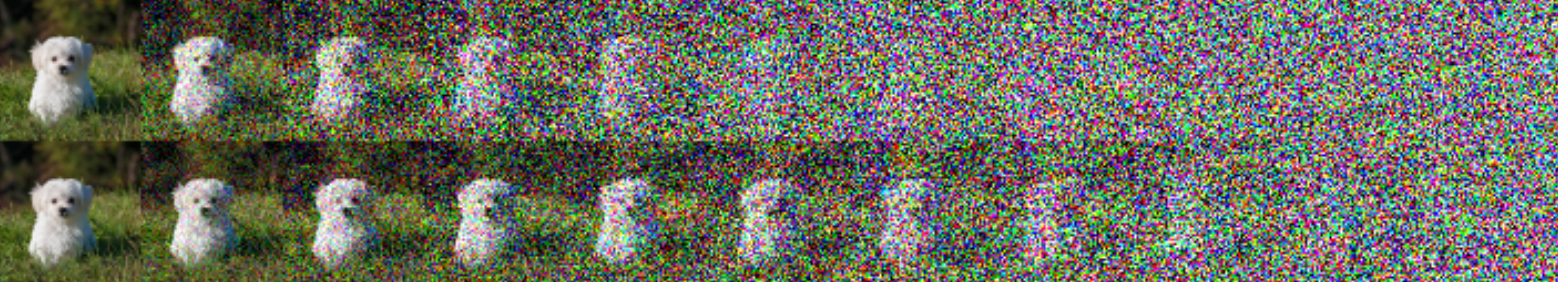
\includegraphics[width=0.9\textwidth]{images/cosine.png}
    \caption[Noising Schedule]{Latent samples from a linear noising schedule (top) and from the proposed cosine schedule (bottom) \cite[Figure 3, p. 4]{nichol2021ImprovedDenoisingDiffusion}}
    \label{fig:cosine}
\end{figure}

A significant milestone for diffusion models was done by \cite{dhariwal2021DiffusionModelsBeat}, where the authors were able to show that diffusion models are able to outperform \gls{gan}
models on image synthesis, which have been considered state-of-the-art at that time \cite{dhariwal2021DiffusionModelsBeat}.
The authors state:

\begin{quotation}
    "We hypothesize that the gap between diffusion models and GANs stems from at least two factors: 
    first, that the model architectures used by recent GAN literature have been heavily explored and refined; 
    second, that GANs are able to trade off diversity for fidelity, producing high-quality samples but not covering the whole distribution. 
    We aim to bring these benefits to diffusion models, first by improving model architecture and then by devising a scheme for trading off diversity for fidelity. 
    With these improvements, we achieve a new state-of-the-art, surpassing GANs on several different metrics and datasets." \cite[p. 2]{dhariwal2021DiffusionModelsBeat}
\end{quotation}


Thus, they argue that \gls{gan} models received more attention, and, therefore, much more improvements in their architecture as well as their training have been discovered, leading to their superior performance.
Furthermore, similar improvements on diffusion models would show that they are able to outperform \gls{gan} models.
These improvements include:
First, several architectural improvements \cite[section 3]{dhariwal2021DiffusionModelsBeat} and an introduction of a classifier guidance mechanism for conditioning \cite[section 4]{dhariwal2021DiffusionModelsBeat}.
Architectural changes include the adding of residual blocks, additional attention mechanisms at different layers, adaptive group normalization, and adding class embeddings into residual blocks \cite{dhariwal2021DiffusionModelsBeat}.
To further improve the conditioning mechanism, \ie controlling what class the model will generate, an additional classifier is introduced \cite{dhariwal2021DiffusionModelsBeat}. 
This classifier is trained on noisy images at different timesteps and is tasked to predict the class of the input image.
During sampling, the gradients produced by this classifier are used by the diffusion model to guide it towards creating an image of that class\footnote{The class of an image depends on the specific dataset. A typical example would be a dataset of animals, where the class of the image would be the name of the animal, \eg a photo of a dog would be of class "dog".} \cite{dhariwal2021DiffusionModelsBeat}.
With these improvements, the authors outperformed \gls{gan} models on unconditional and class-conditional image generation.
Additionally, their model can be controlled in terms of diversity or fidelity through scaling of the classifier guidance gradients.

Since classifier guidance, as presented above, requires training of an additional classifier and thus, increasing the time for computation, \cite{ho2022ClassifierFreeDiffusionGuidance}
introduced a mechanism to achieve a guidance mechanism without an additional classifier.  
Their guidance mechanism is based on the idea of jointly training a conditional diffusion and an unconditional diffusion model and interpolating between their gradients to control the amount of guidance for the output \cite{ho2022ClassifierFreeDiffusionGuidance}.
% The model achieves a trade-off between diversity and fidelity through the adjustments of weights that control the mixing of two metric score estimates of the unconditional and conditioning diffusion model, controling \cite{ho2022ClassifierFreeDiffusionGuidance}.

All the above models apply the diffusion process on the pixel space, resulting in large tensors that require more computation time and require large \glspl{gpu} for computation \cite{rombach2022HighResolutionImageSynthesis}.
\cite{rombach2022HighResolutionImageSynthesis} addresses this issue by moving the diffusion process from the pixel to a latent space.
In the first step, the encoder part of an autoencoder (see \autoref{ch:preliminaries-variationalAutoencoders}) is trained to learn a latent representation with smaller dimensionality of the input image \cite{rombach2022HighResolutionImageSynthesis}.
Given the encoded latent representation, a decoder is tasked to reconstruct the original input.
\autoref{fig:latent-diff} shows the architecture of the overall latent diffusion model \cite[Figure 3, p.4]{rombach2022HighResolutionImageSynthesis}.
The raw input $x$ is encoded into a latent vector $z$ through the pre-trained encoder \cite{rombach2022HighResolutionImageSynthesis}.
Inside this latent space, the diffusion with forward and reverse noising process is performed \cite{rombach2022HighResolutionImageSynthesis}.
Additional conditioning information can be added by transforming the conditioning input into the latent space as well ($\tau_\theta$) \cite{rombach2022HighResolutionImageSynthesis}.
The denoising model is changed compared to previous approaches through the addition of cross-attention blocks to further enhance the generation quality \cite{rombach2022HighResolutionImageSynthesis}.
After the denoising is completed, the pre-trained decoder moves the latent diffusion model output back into the pixel space, generating an image \cite{rombach2022HighResolutionImageSynthesis}.

\begin{figure}[h]
    \centering
    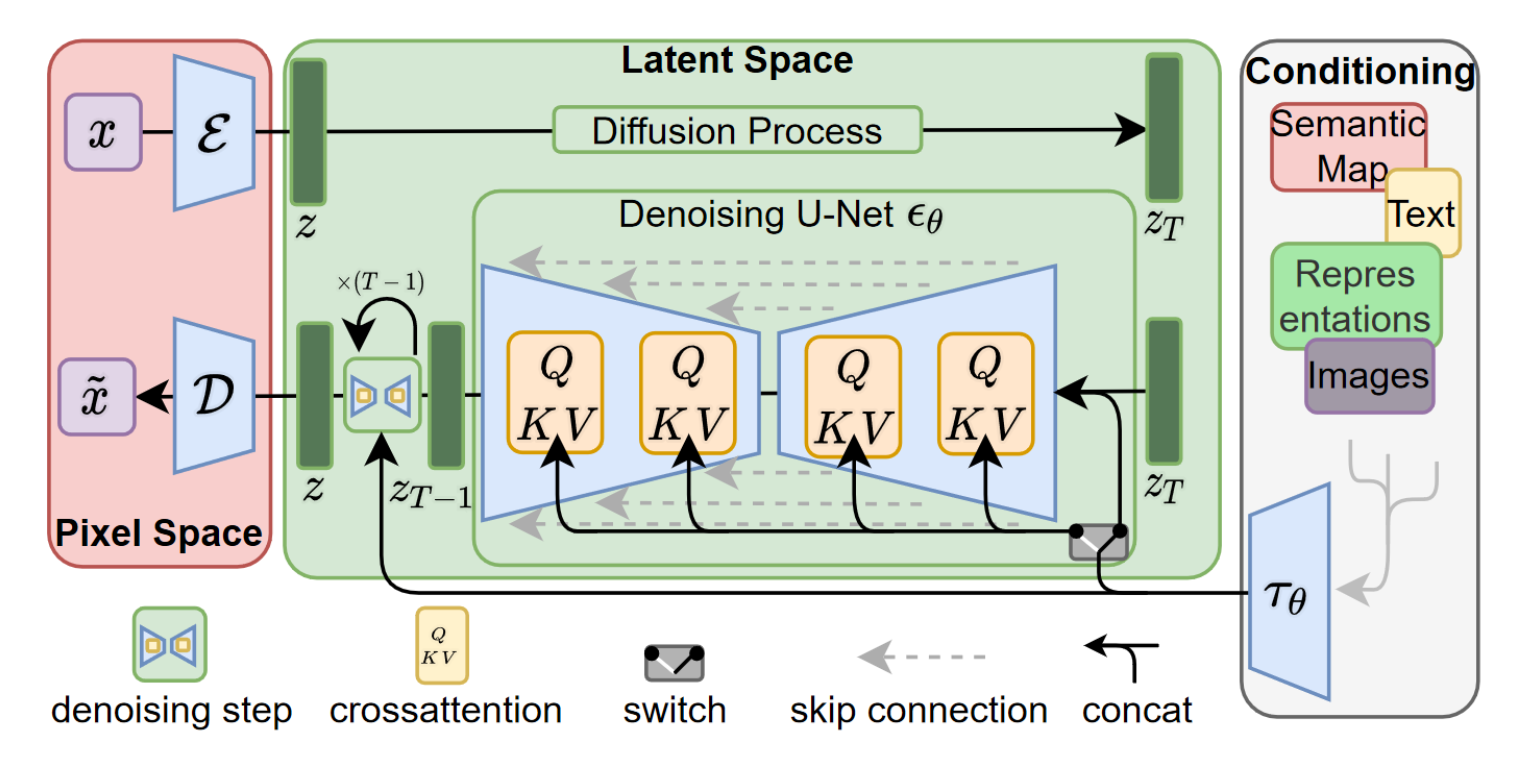
\includegraphics[width=0.9\textwidth]{images/latent-diff.png}
    \caption[Latent Diffusion Model]{Latent diffusion model architecture \cite[Figure 3, p.4]{rombach2022HighResolutionImageSynthesis}}
    \label{fig:latent-diff}
\end{figure}

Thanks to the authors of \cite{rombach2022HighResolutionImageSynthesis} and Huggingface \cite{huggingface2023HuggingFaceAI}, the latent diffusion model was made publicly available and a
pipeline-framework was developed, allowing developers to build upon the existing work easily, test the models locally, and explore and implement new features \cite{huggingface2023DiffusersPipelines}.
This step has led to various community-build diffusion models, ranging from an image-to-image inpainting\footnote{Image-to-image inpainting is a process in computer vision where missing or corrupted parts of an image are filled in with plausible content, usually based on the surrounding context of the image.} diffusion model to a text-to-image diffusion model with multilingual support \cite{huggingface2023CommunityExamples}.

\subsection{Diffusion Probabilistic Models for Tabular Data}
\label{ch:preliminaries-generativeAlgorithms-diffusionProbabilisticModelsTabularData}
At the time of writing, there has been limited work on applying diffusion models to tabular data.
Nevertheless, this section will cover two research papers that apply diffusion to tabular data.

\subsubsection{Diffusion on tabular data imputation}

\textcite{tashiro2021CSDIConditionalScorebased} proposed a conditional score-based diffusion model (CSDI) for the time series imputation task, \ie the task of estimating and filling in missing or absent data points within a time series dataset based on the existing data.
Their CSDI model shows a significant performance increase in generating time-series data compared to other imputation techniques.
\cite{zheng2022DiffusionModelsMissing} showed how the CSDI model can be used in the context of missing value imputation in tabular data that is not a time series (CSDI\_T).
The authors address the problem of simultaneously handling numerical and categorical variables in their work.
Their diffusion model does not reconstruct the complete original data point (\eg an entire tabular data row). 
Instead, the diffusion model receives a splitted version of the input, one part that is observable ("conditional part") $x^{co}$ and one part that is unobservable ("target part") $x^{ta}$.
The goal of the model is, given the unnoised observed part and the noised version of the unobserved part, to return the denoised unobserved part of the next timestep, 
\ie $p_\theta(x^{ta}_{t-1}|x^{ta}_{t},x^{co}_{0})$ \cite{zheng2022DiffusionModelsMissing}.
Categorical entries are converted in three different ways to handle them in conjunction with numerical values.
Categorical values are either \gls{oh} encoded, analog-bits encoded (also called binary encoded), or embedded through a feature tokenization approach proposed by \cite{gorishniy2021RevisitingDeepLearning}.
In the embedding encoding approach, numerical values are encoded as well. 
However, during training, neither the categorical nor the numerical embeddings are learned and remain static and fixed \cite{zheng2023DiffusionModelsMissing}
The authors observed that diffusion achieves the best evaluation metric result for the task of missing value imputation for the tested datasets \cite{zheng2022DiffusionModelsMissing}.
The different encoding techniques perform comparably well, with the embedding technique outperforming the other two techniques by a slight margin \cite{zheng2022DiffusionModelsMissing}.


\subsubsection{Diffusion on tabular data synthesis}
\label{ch:relatedWork-diffusionModels-tabDDPM}

The task of synthesizing an entire tabular dataset through diffusion has been only explored by \textcite{kotelnikov2022TabDDPMModellingTabular}.
The authors introduce their diffusion model, called TabDDPM, for tabular data synthesis, outperforming the existing state-of-the-art approaches using alternative architectures like \glspl{gan} or \glspl{vae} \cite{kotelnikov2022TabDDPMModellingTabular}. 
Since the TabDDPM approach will be the base for this thesis, it will be explained in detail in this section.

Like \textcite{zheng2022DiffusionModelsMissing}, \textcite{kotelnikov2022TabDDPMModellingTabular} identifies the need for processing categorical variables in some form so that they can be processed by a diffusion model.
However, TabDDPM takes a different approach than the CSDI model, using two different diffusion processes.
The classical Gaussian diffusion process \cite{ho2020DenoisingDiffusionProbabilistic} for numerical columns and multinomial diffusion \cite{hoogeboom2021ArgmaxFlowsMultinomial} (\autoref{ch:multinomial}) for categorical/binary columns \cite{zheng2022DiffusionModelsMissing}.
Firstly, the feature columns are preprocessed.
Numerical features are transformed using the Gaussian quantile transformation (\autoref{sec:dataNormalization}), and categorical features are \gls{oh} encoded (\autoref{sec:dataTransformation}) \cite{kotelnikov2022TabDDPMModellingTabular}.
The objective function is defined as:

\begin{equation}
    \label{eqn:tabddpm_loss}
    \begin{align*}
        L^{TabDDPM}_{t} =L^{simple}_t + \frac{\sum_{i \leq C}^{}L^i_{t}}{C}
    \end{align*}
\end{equation}

where $L^{simple}_t$ is equivalent to \autoref{eqn:l_simple} and $L^i_{t}$ being the \gls{kl}-divergence for each multinomial diffusion term ($L_{t-1}$ in \autoref{eqn:vlb3}) divided by the number of categorical features $C$ \cite{kotelnikov2022TabDDPMModellingTabular}.

The neural network used to predict the noise in the reverse process is a simple \gls{mlp} based upon the works of \cite{gorishniy2021RevisitingDeepLearning}.
The architecture consists of several identical \gls{mlp}-blocks comprising a Linear layer, followed by an activation layer (\gls{relu}), and a final dropout layer. 
As in \cite{nichol2021ImprovedDenoisingDiffusion, dhariwal2021DiffusionModelsBeat}, the authors combine the input $x_{in}$ with a sinusoidal temporal embedding\footnote{An encoding of the current timestemp in the diffusion process, computed using the mathematical sine function} and a class label embedding.
Firstly, the input is sent through a linear layer and combined with the temporal and class label embeddings.
The output of that process is sent through a specified number of identical \gls{mlp}-blocks specified above before passing a last linear layer \cite{kotelnikov2022TabDDPMModellingTabular}.

TabDDPM is compared against several baseline models including TVAE \cite{xu2019ModelingTabularData}, CTABGAN \cite{zhao2021CTABGANEffectiveTablea}, CTABGAN+ \cite{zhao2022CTABGANEnhancingTabular},
and a classical interpolation-based approach \gls{smote} \cite{chawla2002SMOTESyntheticMinority}.
Fifteen datasets have been used for generating synthetic data, of which six have a regression task type, seven are binary classification tasks, and two are multiclass classification tasks \cite{kotelnikov2022TabDDPMModellingTabular}.
Eight of the datasets have numerical and categorical features, and seven only consist of numerical features \cite{kotelnikov2022TabDDPMModellingTabular}.
The overall number of features in the datasets varies heavily. 
For a complete list of all datasets, please refer to "Table 2" in \cite[p. 5]{kotelnikov2022TabDDPMModellingTabular}.

The primary evaluation metric chosen by the authors is the machine learning efficacy (see \autoref{ch:preliminaries-machineLearningEfficacy}).
\textcite{kotelnikov2022TabDDPMModellingTabular} realizes this in three different ways, firstly, by using a set of machine and deep learning models\footnote[1]{Decision Tree, Random Forest, Logistic Regression, \gls{mlp}} and averaging their performance,
secondly, using a CatBoost model \cite{prokhorenkova2018CatBoostUnbiasedBoosting}(a state-of-the-art model on tabular tasks) \cite{kotelnikov2022TabDDPMModellingTabular}, and thirdly, an \gls{mlp} architecture proposed by \cite{gorishniy2021RevisitingDeepLearning}.
In the latter case, the models are previously tuned on the real dataset so that the best hyperparameters can be found for each dataset, which will be used during the evaluation \cite{kotelnikov2022TabDDPMModellingTabular}.
To account for other random factors that could influence the results, the authors compute the machine learning efficacy metric scores by generating five different synthetic datasets and train the evaluation models for ten random initializations.
The average over all these 50 variations is reported (\cite[Table 3, 4, p. 8]{kotelnikov2022TabDDPMModellingTabular}) including the standard deviation across the metric results \cite{kotelnikov2022TabDDPMModellingTabular}.
The authors summarize three major findings \cite{kotelnikov2022TabDDPMModellingTabular}:
\begin{itemize}
    \item TabDDPM outperforms TVAE and CTABGAN+ on most datasets.
    \item The classical approach\gls{smote}shows surprisingly competitive performance.
    \item The authors contend that the second evaluation protocol, which employs a state-of-the-art model such as CatBoost, is more suitable for calculating the machine learning efficacy, 
    despite the prevalent use of the first protocol in prior works. 
    The firstly mentioned set of models shows overall lower metric scores compared to the CatBoost model.
    Thus, the authors argue their performance values are uninformative.
    Additionally, for the set of models, the models trained on synthetic data outperformed the models trained on actual real data, indicating that the 
    synthetic data is "more valuable than the real" data, which should not be the case \cite[p. 8]{kotelnikov2022TabDDPMModellingTabular}.
    This behavior cannot be observed if tuned \gls{mlp} or CatBoost models are used for evaluation \cite{kotelnikov2022TabDDPMModellingTabular}.
\end{itemize}

Additionally, the authors provide a small comparison based on distribution plots and correlation matrices.
In their comparison, they show that the produced feature distribution plots by TabDDPM for a selected number of columns of different datasets look more similar 
to the real distributions, compared to plots produced by CTABGAN+ or TVAE \cite{kotelnikov2022TabDDPMModellingTabular}.
The authors argue that this observation is consistent for numerical, categorical, and mixed data type columns \cite{kotelnikov2022TabDDPMModellingTabular}.
The pairwise correlation matrices difference plots (performed similarly to in \cite{brenninkmeijer2019GenerationEvaluationTabular}) show a smaller difference between the synthetic and real data for the TabDDPM model compared to CTABGAN+ and TVAE.
The authors assert that the illustrations provided demonstrate that their TabDDPM model exhibits greater flexibility than other alternatives and generates synthetic data of higher quality \cite{kotelnikov2022TabDDPMModellingTabular}.

Lastly, \cite{kotelnikov2022TabDDPMModellingTabular} performs a privacy evaluation against the\gls{smote}approach.
The median \gls{dcr} is, which calculates the minimum Euclidean distance to real data points for each synthetic sample \cite{zhao2021CTABGANEffectiveTable}.
Small \glspl{dcr} point towards mere copying of data samples (overfitting), while high values indicate actual new synthetic data samples \cite{kotelnikov2022TabDDPMModellingTabular}.
The results presented by the authors show a higher \gls{dcr} score for TabDDPM for all datasets compared to\gls{smote}while having a similar or higher machine learning efficacy score \cite{kotelnikov2022TabDDPMModellingTabular}.

To summarize, the TabDDPM approach is a novel way to generate synthetic data of high utility using Gaussian and multinomial diffusion.
TabDDPM outperforms other state-of-the-art baseline models in terms of machine learning efficacy on multiple datasets.
Moreover, distributions and correlations produced from synthetic data by TabDDPM look more similar to the real data than synthetic data produced by other models.





